
\noindent
Integrating curvilinear geometries into modelling software is an involved multi-level process. It requires meshing software capable of creating accurate higher order elements from analytic designs or experimental data, curvilinear grid manager able to efficiently manipulate such elements, as well as a PDE solver able to benefit from the curved geometries. The latter is mainly achieved by means of curvilinear basis functions able to accurately describe the associated vector field (e.g. div or curl-conforming), adapting to the non-linear "bending of space". Ideas of using curvilinear grids first appeared in the literature in the 1970s \citep{ciarlet+1972, lenoir1986} and have been used in electromagnetic simulations for at least two decades \citep{wang+1993}. \\

%%
\noindent
A impressive example of using a curvilinear $3$-dimensional code together with DG and optimized for parallel GPU processing can be found in the aerodynamics community (\citeauthor{Warburton2012}).
%%
\citeauthor{wang+2011} demonstrate a 3D curvilinear parallel DG code for solving Maxwell's equations in a homogeneous medium.
%%
Still, they are much less widespread than linear meshes and so far have only been explicitly presented in 2D codes \citep{wang+2011a}.
%%
Having finished the implementation of a curvilinear code ourselves, we believe that the challenges causing this lack of adoption are as follows:
\begin{itemize}
\item Generation of curvilinear meshes is a challenging process, as naive approaches can easily result in self-intersecting meshes \citep{toulorge+2013, johnen+2012}. Further, it must be ensured that the generated elements are optimal for the optimal PDE convergence \cite{lenoir1986}.
\item Standard functionality of a grid manager, such as interpolation, local-to-global and global-to-local mappings, integration, calculation of normals and basis functions becomes significantly more difficult in curvilinear case, as shown below; additional numerical tools, such as Lagrange interpolation, adaptive integration, analytical polynomials, and optimization algorithms have to be employed to provide the desired functionality. 
\item In order to fully benefit from the curvilinear geometries through reducing the total element count, basis functions of order sufficient to resolve the detailed structure of the field are necessary. The widely used Continuous-Galerkin based codes require a curvilinear higher order basis that preserves field continuity across the element boundary, which appears to be a challenging task. At the moment of writing authors are not aware of publications presenting such a basis. \citeauthor{fahs2011} implements a serial time-domain 2D and 3D curvilinear Discontinuous-Galerkin (DG) code using polynomially-complete basis and studies the scaling of the accuracy of electromagnetic benchmarks (\textit{Mie} scattering and layered \textit{Mie} scattering) depending on p-refinement. He finds that only in curvilinear geometries increasing the basis function order significantly improves the solution accuracy.
\end{itemize}

\noindent
To the best of our knowledge, the combination of higher order curvilinear meshes and domain decomposition has not yet appeared in a parallel DG frequency-domain code. Until recently, literature presents implementations of such codes with several simplifications, limiting the the flexibility and detail achievable on moderate computational resources. \\

\noindent
Nevertheless, higher order geometries carry large potential. The fundamental target is to improve the accuracy of the solution given a fixed computational resource, and curvilinear geometries can offer that. The curvilinear material boundaries have smooth corners unlike their linear analogues \cref{fig:result:spherecurv}, avoiding the unphysical "corner effects" (such as unexpected highly localised field enhancement), which otherwise have to be treated by high h-refinement. \\

\begin{figure}
    \centering
	\begin{subfigure}[b]{0.48\textwidth} \hspace{8mm} 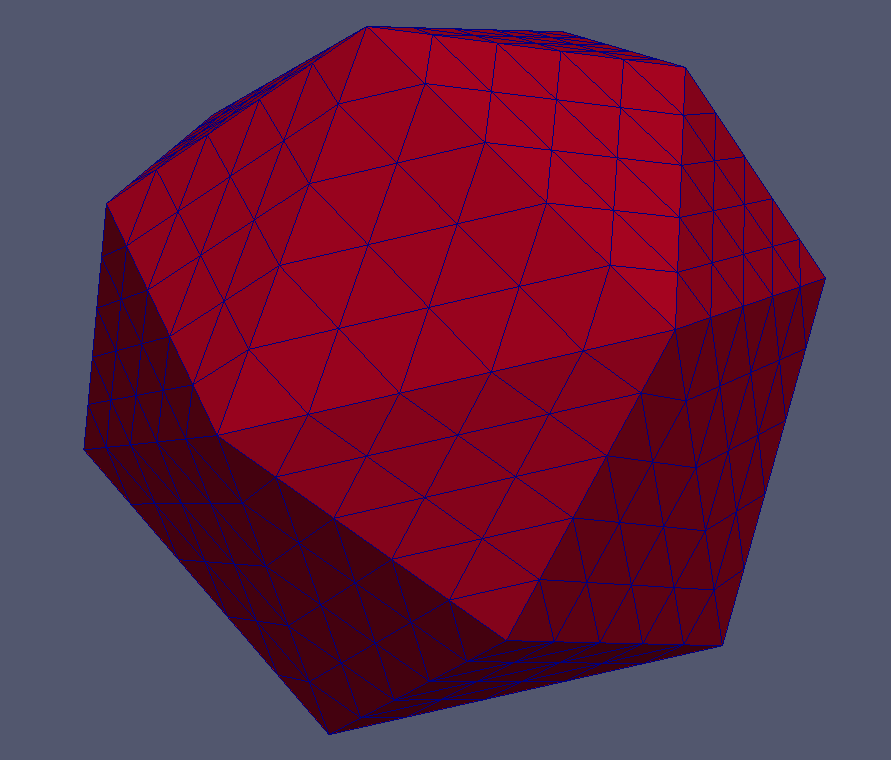
\includegraphics[scale=0.215]{images/sphere32discr6ord1} \end{subfigure}
	\begin{subfigure}[b]{0.48\textwidth} 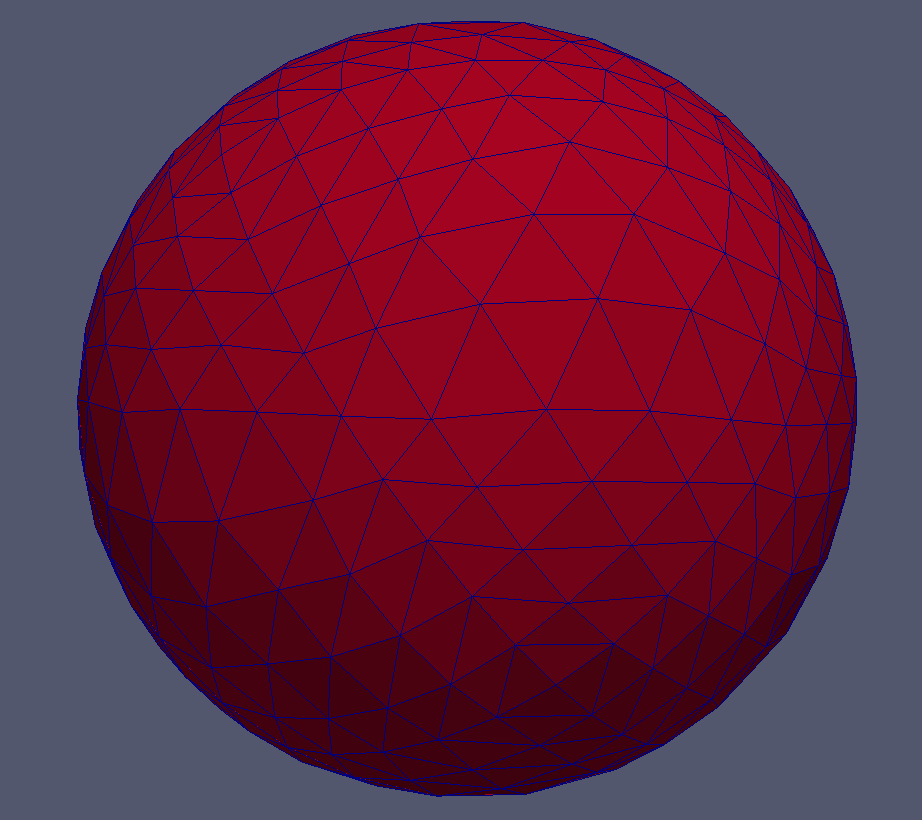
\includegraphics[scale=0.2]{images/sphere32discr6ord5} \end{subfigure}
	\captionsetup{width=0.8\textwidth} 
	\caption{Presented is the 32 element tetrahedral mesh of a sphere, using first and fifth order polynomial interpolation. Visualisation software (Paraview, in this case) does not appear to have documented interface for direct curvilinear element output. The curvature is represented by virtual refinement of curvilinear tetrahedra into smaller linear tetrahedra }
	\label{fig:result:spherecurv}
\end{figure}

\noindent
Further, the accuracy of a PDE solution improves much faster with increasing basis function order, as opposed to increasing number of elements \cite{jin2014} \cref{fig:jin:basisconv}. However, in case of smooth material boundaries this effect can only be exploited if the corresponding element geometries are of sufficiently high order \cite{fahs2011} \cref{fig:fahs:curvconv}.

\begin{figure}
    \centering
    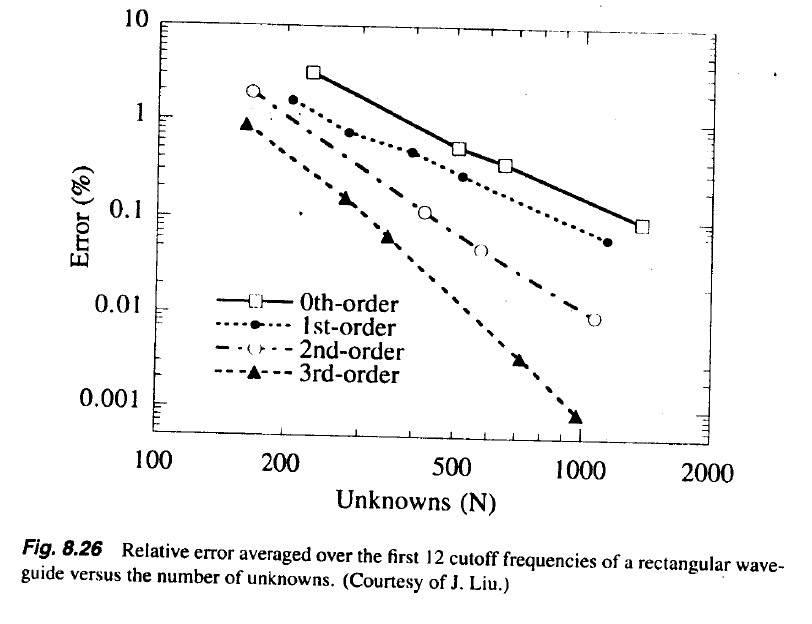
\includegraphics[scale=0.4]{images/Jin-basis-function-efficiency}
	\captionsetup{width=0.8\textwidth} 
	\caption{ \citeauthor{jin2014} shows that the improvement of accuracy due to h-refinement improves exponentially with increasing basis polynomial order }
	\label{fig:jin:basisconv}
\end{figure}

\begin{figure}
    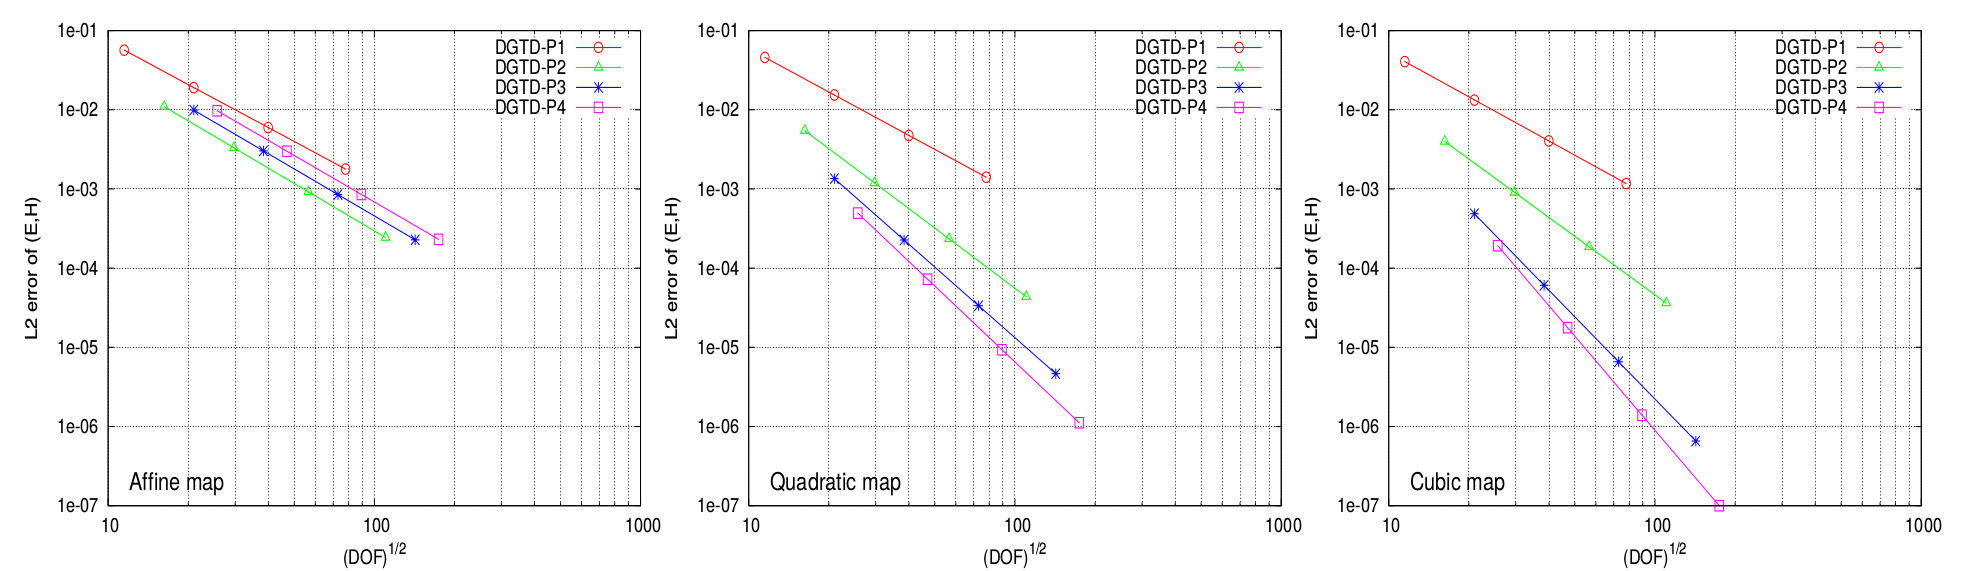
\includegraphics[scale=0.25]{images/fahs-convergence}
	\captionsetup{width=0.8\textwidth} 
	\caption{ \citeauthor{fahs2011} shows that computational accuracy (in terms of $L_2$ error) improves with increasing basis function order, but it improves faster if the entity interpolation (curvature) order is increased accordingly}
	\label{fig:fahs:curvconv}
\end{figure}


\section{Capabilities of CurvilinearGrid}
\label{section-outline-capabilities}

The Curvilinear Grid (CurvGrid) is a self-consistent grid manager supporting 3D tetrahedral curvilinear grids. It depends on the core modules of Dune \citeDune{}, as well as an external parallel mesh partition library Parmetis \citeParMetis{}. Also, CurvGrid depends on Curvilinear Geometry (CurvGeom), also developed by us as a separate dune-module. \\

\noindent
CurvGeom is capable of interpolating and performing multiple geometric operations over curvilinear simplex entities (edges, triangles and tetrahedra) of orders 1-5 via hard-coded Lagrange Polynomials, and arbitrary order simplex entities via analytic Largange Interpolation method. CurvGeom complies with standard dune-geometry interface, providing methods for local-to-global and global-to-local coordinate mapping, computation of Jacobian matrix, integration element and entity volume. CurvGeom has a non-cached and cached implementations, where the cached version pre-computes the local-to-global map and its determinant, thus performing considerably faster for integration and mapping tasks. In comparison with standard dune-geometry, CurvGeom provides methods to obtain either all interpolatory vertices of an entity or only its corners, as well as the method to obtain the curvilinear order. Additionally, CurvGeom provides the methods to obtain outer normals of subentities of the geometry, and the subentity geometries themselves. An additional feature of CurvGeom is the analytical polynomial class and associated differential methods, which allow to obtain analytical expressions for local-to-global map and associated integration element, enabling exact manipulation of geometries of arbitrary order. CurvGeom contains its own recursive integration tool, wrapping the quadrature rules provided by dune-geometry. The reason for implementing this functionality is to accurately treat non-polynomial integrands, for which the optimal polynomial order for desired accuracy is not known. In particular, it happens that curvilinear integration elements are non-polynomial in general case (see \cref{sec:theory:integration}). The recursive integration scheme is able to simultaneously integrate multidimensional integrands, such as vectors and matrices. This is highly useful, for example, for integrating outer product matrices where evaluation of all matrix elements at a given point only requires $O(N)$ expensive function evaluations. CurvGeom also provides a utility for testing curvilinear entities for self-intersection by sampling the value of integration element across the entity. \\

\noindent
CurvGrid module manages the entire process of parallel reading, manipulating, and writing of curvilinear geometries and associated fields (e.g. PDE solution). The former is performed by Curvilinear GMSH Reader (CurvReader). CurvReader is currently capable of reading curvilinear \textit{.msh} files of orders 1 to 5, where 1 corresponds to linear meshes. CurvReader is highly parallel-scalable, meaning that each process only reads the necessary local part of the mesh, avoiding memory overflow. CurvReader has the option to partition the mesh using ParMetis during the reading procedure before reading the curvature vertices, further decreasing the file access time. CurvReader also reads material elementary and boundary tags provided GMSH. It extends the standard Grid Factory interface, providing tag information, as well as curvilinear order. The grid output is performed by Curvilinear VTK Writer (CurvWriter) module, supporting VTK, VTU and PVTU file formats. CurvWriter can either write the entire grid automatically, or write a set of individual entities, provided one at a time. When writing the entire grid, each element is supplied by fields denoting its rank, partition type and physical tag, which can be used to visually inspect the parallel connectivity of the domain \cref{fig:result:spherestruct}. The scalability of the grid assembly and visualisation has been tested on instances with 12 to 128 cores using the multiple geometries, the largest being the 4.4 million element tetrahedral mesh \cref{fig:result:bullseye}. The user has full flexibility to define the codimensions of the entities that will be written, the choice to write interior, domain, process boundaries and/or ghost elements, as well as the order of virtual refinement of curvilinear entities. The output mesh can be supplied with arbitrary number of vector and scalar fields representing, for example, the solution(s) of a PDE. We have tested the visualisation capabilities of CurvGrid using ParaView \cite{johnson+2005} and VisIt \cite{childs+2012} end user software. \\

\begin{figure}[H]
	\begin{subfigure}[b]{0.30\textwidth} \hspace{4mm} 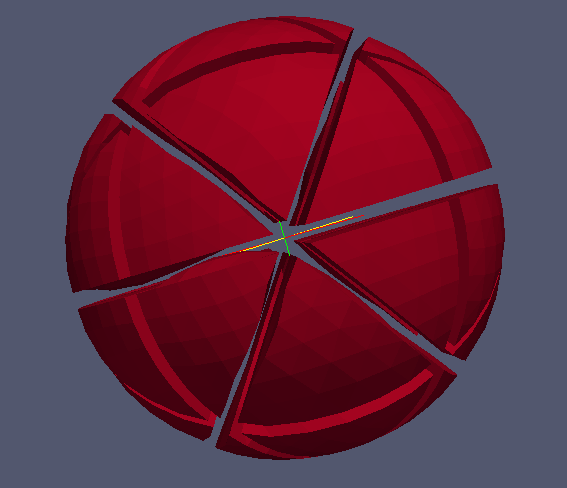
\includegraphics[scale=0.22]{images/32-inter} \captionsetup{width=0.8\textwidth} \caption{ Interior Elements } \end{subfigure}
	\begin{subfigure}[b]{0.30\textwidth} \hspace{4mm} 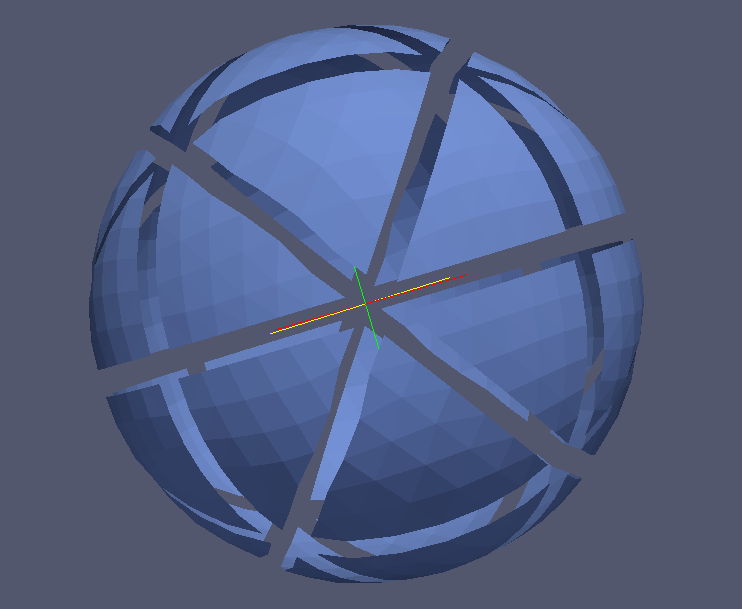
\includegraphics[scale=0.18]{images/32-db}    \captionsetup{width=0.8\textwidth} \caption{ Domain Boundaries} \end{subfigure}
	\begin{subfigure}[b]{0.33\textwidth} \hspace{4mm} 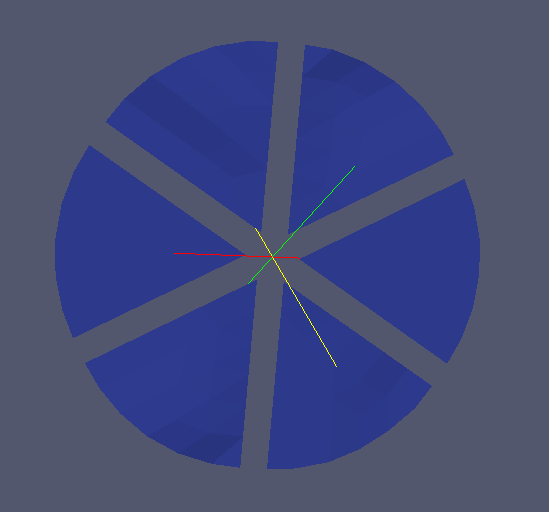
\includegraphics[scale=0.22]{images/32-pb}    \captionsetup{width=0.8\textwidth} \caption{ Interprocessor Boundaries} \end{subfigure}
	\begin{subfigure}[b]{0.46\textwidth} \vspace{5mm} \hspace{12mm} 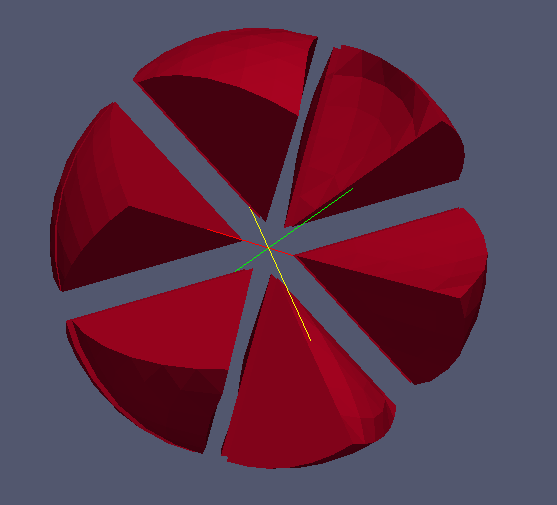
\includegraphics[scale=0.25]{images/32-ghost} \captionsetup{width=0.6\textwidth} \caption{ Ghost Elements} \end{subfigure}
	\begin{subfigure}[b]{0.46\textwidth} \vspace{5mm} \hspace{12mm} 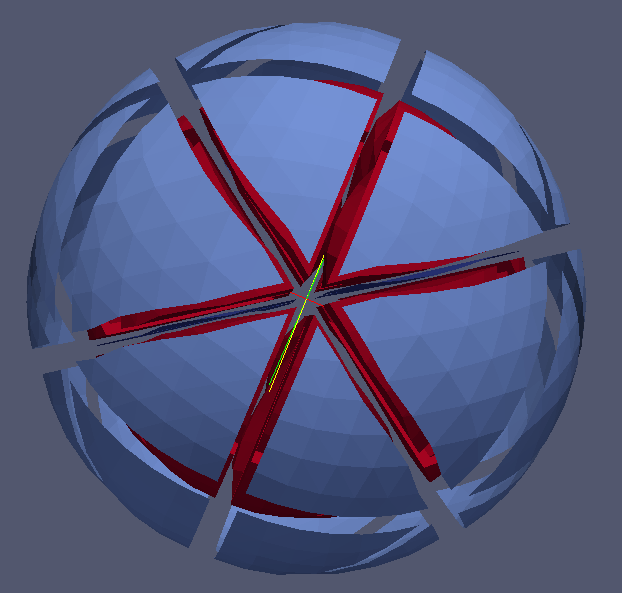
\includegraphics[scale=0.21]{images/32-full}  \captionsetup{width=0.6\textwidth} \caption{ Entities of all structural types visualised at the same time } \end{subfigure}
	\caption{ Visualisation of various structural (partition) types of a 32 element tetrahedral mesh, loaded in parallel on 2 cores }
	\label{fig:result:spherestruct}
\end{figure}

\begin{figure}[H]
    \centering
	\begin{subfigure}[b]{0.48\textwidth} 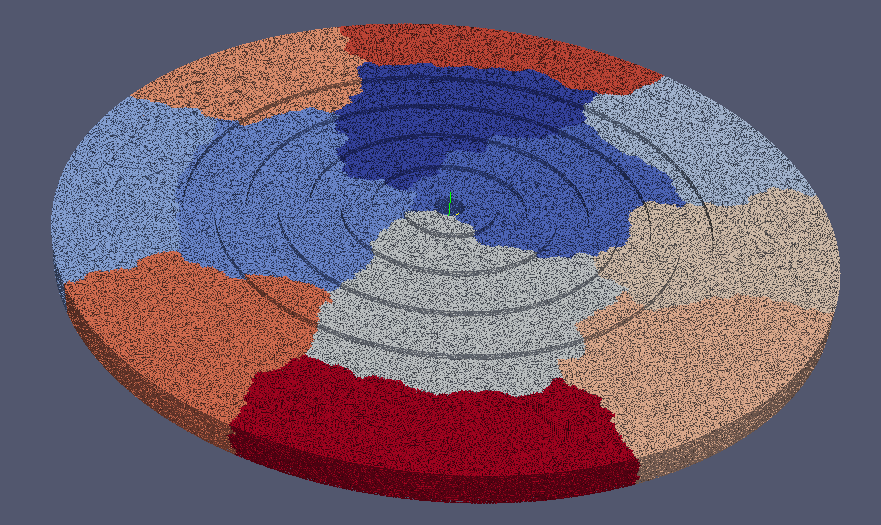
\includegraphics[scale=0.20]{images/bullseye-core-angle}          \captionsetup{width=0.8\textwidth} \caption{Interior elements coloured by owner process rank}   \end{subfigure}
	\begin{subfigure}[b]{0.48\textwidth} 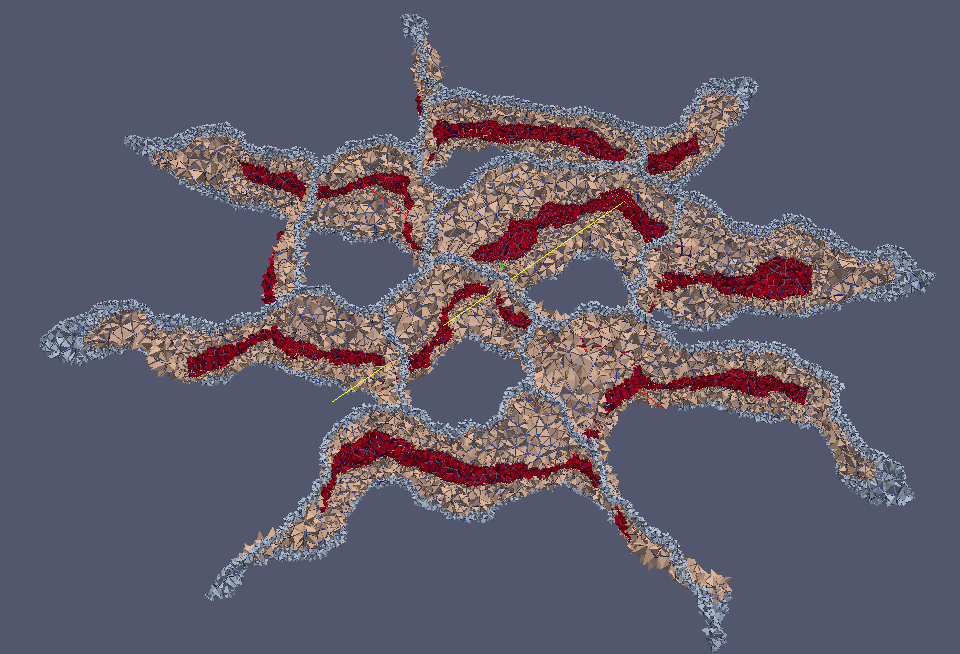
\includegraphics[scale=0.17]{images/bullseye-ghostelements-angle}  \captionsetup{width=0.8\textwidth} \caption{Ghost elements, coloured by material tag} \end{subfigure}
	\caption{Interior and ghost elements of a 4.4 million element tetrahedral mesh of the Bullseye geometry}
	\label{fig:result:bullseye}
\end{figure}

\noindent
The core of CurvGrid provides essential indexing and communication capabilities. Global and local index is provided for all codimension entities. The interprocessor communication is performed via the dune standard DataHandle interface for provided Ghost elements entities of all codimensions. In extension to dune-grid interface, it is possible to directly address the core curvilinear geometry of each entity, as well as the associated physical tags. CurvGrid is also equipped with a set of useful utilities:
\begin{itemize}
    \item Timing mechanisms, implementing parallel timing of separate parts of code with following statistics output over all processes
    \item Logging mechanisms, implementing real time logging of current state of the code, as well as the current memory consumption on each core of the machine, allowing for real-time diagnostics of memory bottlenecks of the code.
    \item Nearest neighbour communication, wrapping the MPI-2 implementation of \textit{MPI\_Neighbor\_alltoall} for vector communication with neighboring processes. \textbf{[CITE ME]}
    \item Global boundary container, implementing interior/domain boundary all-to-all communication, useful for dense PDE solvers, such as the Boundary Integral method. \cite{kern+2009}
    \item Grid diagnostics, collecting statistics on entity volume, quality and distribution among processes
\end{itemize}

\noindent
We also present the major TODO list. This functionality is currently NOT available in the CurvGrid, but is desirable to have. We welcome contributions from the community \\

\noindent
\begin{tabularx}{\textwidth}{l X}
\hline
     Difficulty & Description \\
\hline
	 Easy & Using GMSH partition tags to read pre-partitioned meshes \\
	 Easy & CurvReader extension to arbitrary order curvilinear simplex geometries. Involves writing an abstract mapper from GMSH to sorted cartesian node indexing. \\
	 Medium & Multi-constraint grid partition by CurvReader able to, for example, provide processes with contiguous grid parts with balanced element and boundary segment count. \\
	 Medium & Dynamic load balancing \\
	 Medium & Complete CurvGrid optimization for high parallel scalability using nearest neighbour communication \\
	 Medium & Non-uniform polynomial order curvilinear meshes \\
	 Medium & Efficient location of the curvilinear element containing a given global coordinate (for example, via Octant Tree) \\
	 Medium & Identification and management of periodic boundaries directly from boundary tags \\
	 Medium & 1D and 2D curvilinear simplex grids \\
	 Medium & Front/Overlap partition types \\
	 Hard & Other geometry types (for example, hexahedral geometries) \\
	 Hard & Mixed element grids \\
	 Hard & Non-conformal curvilienar meshes (with hanging nodes) \\
	 Hard & Global and local refinement of curvilinear grids, including adaptive refinement \\
\hline
\end{tabularx}

%%%\section{Design decisions}
%%%\label{section-outline-designdecisions}
%%%
%%% Design decisions for Curvilinear Grid Factory
%%%\begin{itemize}
%%%	\item User must provide globalId's for vertices and elements. [Automatically implemented by GMSH \citeGMSH]
%%%	\item User must provide all boundary segments inside GMSH file.
%%%\end{itemize}


\section{Internal Structure}
\label{section-outline-internalstructure}

Below we present a simplified structure of classes used by Curvilinear Grid and geometry \\

\noindent
\begin{tabularx}{\textwidth}{ l | X }
\hline
   Class Name & Description \\ \hline
   CurvilinearGeometry                & Core class complying with dune-geometry standard \\ \hline
   * CurvilinearGeometryHelper        & Auxiliary functions, subentities for curvilinear elements \\ \hline
   * LagrangeInterpolator             & Lagrange Interpolation of element geometry \\ \hline
   * Polynomial                       & Analytic polynomial routines \\ \hline
   * DifferentialHelper               & Analytic Curvilinear Jacobians and Integration elements \\ \hline
   * IntegralHelper                   & Integral Functors, analytic integration routines  \\ \hline
   * QuadratureIntegrator             & Recursive integration using numerical quadrature. Performs fast \\ \hline
   * AdaptiveIntegrator               & Recursive integration using adaptive refinement. Performs slowly \\ \hline
  CurvilinearGMSHReader               & Reads a $.msh$ file and supplies entities to a Grid Factory \\ \hline
  * Gmsh2DuneMapper                   & Converts between interpolation vertex numbering paradigms \\ \hline
  CurvilinearVTKWriter                & Writes curvilinear elements to VTK, VTU/PVTU files \\ \hline
  CurvilinearVTKGridWriter            & Writes Curvilinear Grid to VTK, VTU/PVTU files \\ \hline
  CurvilinearGridBase                 & Lower level grid implementation. All entities are given by their codimension and index \\ \hline
  * CurvilinearGridStorage            & Storage class for entire grid \\ \hline
  * CurvilinearGridConstructor        & Constructs entities of the grid, finds neighbouring processes, generates global index \\ \hline
  * CurvilinearGhostConstructor       & Constructs ghost entities \\ \hline
  * CurvilinearPostConstructor        & Enables DataHandle communication \\ \hline
  Curvilinear Grid                    & Core class complying with dune-grid standard \\ \hline
  * CurvilinearGridFactory            & Interface for constructing Curvilinear Grid \\ \hline
  * CurvilinearGridDiagnostics        & Tests and collects statistics on Curvilinear Grid \\ \hline
  * LoggingMessage                    & Logging output with varying levels of verbosity \\ \hline
  * LoggingTimer                      & Parallel timing of parts of code. \\ \hline
  * AllCommunicate                    & Nearest neighbour communication for POD. Wrapper for $MPI\_alltoallv$ \\ \hline
  * VectorHelper                      & Manipulation of vectors (union, intersection, complement), as well as conversion to string \\ \hline
\end{tabularx}
